\documentclass[a4paper, 11pt]{article}
\usepackage[T1]{fontenc}
\usepackage[utf8]{inputenc}
\usepackage{natbib}
\usepackage{hyperref} % links
\usepackage{multirow} % context example table
\usepackage{array} % fixed-width columns with left alignment
\usepackage{graphicx} % include the map
\usepackage[outline]{contour} % contour place names in the cosine similarity figure
\usepackage[dvipsnames]{xcolor} % colour-code the groups (has to come before tikz)
\usepackage[geometry]{ifsym} % shape-code the groups
\usepackage[section]{placeins} % don't let the graphics/tables move past sections
\usepackage{float} % place figures where I want them
\usepackage{pdfpages} % add non-plagiarism statement (has to be after xcolor)
\usepackage{tipa} % IPA
\usepackage{amsmath} % formulae
\usepackage{dsfont} % real numbers symbol
\usepackage{mathtools} % display style in formulae with branching cases
\usepackage{forest} % (non-dendrogram) trees
\usetikzlibrary{decorations.pathreplacing} % draw braces in tikz figures
\usepackage{standalone} % import figures
\usepackage{changepage} % adjust text width
\usepackage{parskip} % proper paragraphs, no indentation
\usepackage{titling} % Skip authorship information

\usepackage[margin=2.5cm]{geometry}
\linespread{1.25} % GSCL formatting requirement


% For the map keys.
\definecolor{purple}{HTML}{520066}
\definecolor{midblue}{HTML}{31688e}
\definecolor{green}{HTML}{35b779}
\def\upper{\color{purple}\FilledBigTriangleUp}
\def\central{\color{midblue}\FilledBigSquare}
\def\dutch{\color{green}\FilledBigCircle}
\def\ingv{\color{green}\BigCircle}

% For specifying matrix dimensions. (set of real numbers symbol)
\newcommand{\R}{\mathds{R}}

\title{Summary: Clustering Dialect Varieties Based on Historical Sound Correspondences (Bachelor's Thesis)}
% Skip the date
\predate{}
\postdate{}
\date{}
%% Anonymize paper for the GSCL submission:
% \preauthor{}
% \postauthor{}
% \author
\author{Author: Verena Blaschke, Supervisor: Dr. Çağrı Çöltekin}
\setlength{\droptitle}{-2cm}

\begin{document}


% \pagenumbering{arabic}

\maketitle

\section{Introduction}

While information on historical sound shifts
plays an important role for examining
the relationships between related language varieties,
it has rarely been used for computational dialectology.

In this thesis, we examine a set of West Germanic language varieties
currently spoken in continental Europe.
We compare them by investigating how they have changed phonologically
since a shared ancestral stage of Germanic.
Our goal is to automatically assign a cluster structure to the
modern language varieties that reflects shared sound changes
within each cluster and differences between sound shifts between different clusters.
In doing so, we examine the performance of two different clustering algorithms.

% Applying quantitative methods to dialectology gives the advantage
% that statistical models can work using all the feature
% information of the data that they are given,
% quickly evaluating for each feature how well it does or does not
% describe similarities or differences in the data.
% This LINE OF RESEARCH HAS SIMILARLY BEEN CARRIED OUT BY, e.g., 
% \citeauthor{prokic2012detecting} (\citeyear{prokic2007identifying}; \citeyear{prokic2012detecting}; \citeyear{prokic2013combining}),
% \citeauthor{wieling2011bipartite} (\citeyear{wieling2009bipartite}; \citeyear{wieling2010hierarchical}; \citeyear{wieling2011bipartite}),
% \citet{wieling2013analyzing} and \citet{montemagni2013synchronic}.

\section{Continental West Germanic} % Historical and dialectological background?

The continental European West Germanic (henceforth: CWG) language varieties 
(hereafter referred to as \textit{doculects}) include several standard languages
(Luxembourgish, multiple standard varieties of Dutch and German)
as well as many regiolects and dialects.
Establishing subgroups within this collection of doculects provides a challenge
due to their being very similar to one another.

Nevertheless, there are some common ways of grouping CWG doculects into broad sub-groups.
Firstly, they can be divided into Ingv{\ae}onic (Low German and Frisian) and non-Ingv{\ae}onic varieties, based on pronoun systems and morphological and phonological characteristics
(\citet{stiles2013pan-west}; \citet[pp.~7--8]{harbert2007germanic}).

Secondly, 
CWG doculects can be divided into three groups according to
the results of the High German sound shift, a lenition of voiceless (Proto-)Germanic stops to affricates or fricatives:
Upper German (which almost completely
exhibits lenition for all voiceless stops),
Central German (which shows a
partial development of the High German sound shift),
and Low German as well as Dutch and Frisian (which were not influenced by the High German sound shift)
(\citet[pp. 33, 55]{noble1983modern}; \citet[pp.~64,~230--231]{koenig2015dtv}).


\subsection{Data}

We work with phonetically transcribed data from
CWG doculects, taken from the Sound Comparisons project 
\citep{heggarty2018sound}.
We used 110 cognate sets (also referred to as \textit{concepts})
from 20 modern CWG doculects
and a reconstructed version of Proto-Germanic.

The modern doculects are from locations in the
Netherlands, Belgium, Luxembourg, (along the Western border of) Germany,
France (Alsace), Switzerland, Liechtenstein, Austria (Voralberg), and Italy (South Tyrol).
Figure~\ref{fig:map} provides an overview of these locations.

The Proto-Germanic data cover all 110 concepts; each of the modern doculects covers at least 103 concepts, and each concept is covered by at least 17 modern doculects.
In total, we have 2181 word alignments between Proto-Germanic and the modern CWG doculects.


\section{Methods}

We first align the phonetic transcriptions from our data
to then extract sound correspondences, which we use for
two different clustering methods.

\subsection{Multiple Sequence Alignment}

We carry out alignment based on data from
all the investigated doculects at once using multiple sequence alignment.
We use a library-based version \citep{notredame2000t-coffee:} of the progressive multiple sequence alignment method \citep{thompson1994clustal}, as implemented in the LingPy library for Python \citep{list2018lingpy}.

\subsection{Sound Correspondence Extraction}

Next, we extract sound correspondences between
Proto-Germanic and each modern doculect from the alignment tables for all concepts.
We use straightforward segment-to-segment correspondences,
as well as correspondences that include contextual information.
For the latter, firstly, we separately add information about the
left and right single-segment context,
stating whether it is a consonant or a vowel.
This can only be performed when the context in question is of
the same type for both Proto-Germanic and the modern doculect.
Additionally, we repeat the same process, but use the more fine-grained sound class system by \citet{list2012sca}, which recognizes fifteen consonant and six vowel group.
Lastly, we also use sound correspondences that explicitly capture correspondences at word-initial and -final positions.

We ignore gap-gap alignments,
and treat cases of segment swaps (metathesis) as normal insertions or deletions.
For each doculect, we ignore sound correspondences
that occur fewer than three times across all concepts
to reduce the effect misalignments might have. 

After extracting the sound correspondences for
all modern doculects, we have a doculect-by-correspondence
matrix storing the absolute frequencies of the sound correspondences per doculect.

\subsection{Clustering}

We implemented two approaches to custering the data.
Both clustering approaches follow a similar structure:
we first normalize the doculect-by-correspondence tally matrix
to adjust feature frequencies by how informative they are,
then we perform hierarchical clustering.
Each approach is carried out once with only
the context-less sound correspondences,
and once with all context types.

\subsubsection{Agglomerative Clustering}

We first normalize the frequencies
in the doculect-by-correspondence tally matrix
by applying TF-IDF weighting.
% AS IMPLEMENTED in the scikit-learn library \citep{pedregosa2011scikit-learn}.
We calculate the cosine distances between each
binary combination of row vectors from this matrix
to create a doculect-by-doculect distance matrix.

We then convert this distance matrix into a dendrogram using the
Unweighted Pair Group Method using Arithmetic Averages
(UPGMA) method introduced by \citet{sokal1958statistical},
which was found to be well-suited
for analyzing dialect distances by \citet[p. 153]{heeringa2004measuring}
and \citet{prokic2008recognizing}.

Henceforth, we refer to the results of this approach
as \textit{UPGMA-context} and \textit{UPGMA-nocontext}.

\subsubsection{Bipartite Spectral Graph Co-clustering}

For the other clustering method, we perform Bipartite Spectral Graph Co-clustering (BSGC)
\citep{dhillon2001co-clustering},
which was introduced to 
%statistical dialectology 
dialectometry
by \citeauthor*{wieling2009bipartite} (\citeyear{wieling2009bipartite}; \citeyear{wieling2010hierarchical}).

BSGC works by normalizing the doculect-by-correspondence matrix such that all doculects and sound correspondences can be mapped to vectors in the same vector space.
Using k-means clustering with $k=2$, each vector is assigned to one of two clusters. 
For each new cluster, both the normalization and the clustering step are recursively repeated.

Occasionally, it happens that a cluster produced by the k-means clustering step contains a sound correspondence that is not exhibited
by any of the doculects in the same cluster.
In that case, it is not possible to normalize the new cluster's co-occurence matrix, and we therefore need to assign the sound correspondence to the other cluster that was produced in the k-means clustering step.
% TODO verstaendlich schreiben

The results from this method are hereafter referred to
as \textit{BSGC-context} and \textit{BSGC-nocontext}.

\subsection{Ranking Sound Correspondences by Importance}

When all doculects have been assigned to a hierarchical cluster structure,
we rank the sound correspondences associated with each cluster.
These are either
all sound correspondences exhibited by a cluster's doculects (UPGMA),
or the sound correspondences that are in the same cluster (BSGC).

We use the \textit{representativeness} (What proportion of doculects in a given cluster exhibit a given sound correspondence?) and \textit{distinctiveness} (How often does a given sound correspondence occur in a given cluster compared to other clusters?) metrics
introduced by \citet{wieling2011bipartite},
as well as a modified version of their \textit{importance} metric 
(the harmonic mean of representativeness and distinctiveness).
For all metrics, higher values are better; the best possible score is $100 \%$.

\section{Results}

Figures~\ref{fig:tfidf-dendrograms} and \ref{fig:bsgc-trees} visualize the results of UPGMA and BSGC, respectively.

One notable difference between the results of the two methods is the number 
of sound correspondences with importance scores of 100\% 
associated with intermediary clusters
(i.e. clusters that are neither singletons nor contain all doculects):
More sound correspondences associated with UPGMA have perfect importance scores compared to the results of BSGC (UPGMA-nocontext: 6/201 vs. BSGC-nocontext: 1/201; UPGMA-context: 24/665 vs. BSGC-context: 2/665).

Similarly, most (13/18; UPGMA-nocontext) or almost all (17/18; UPGMA-context) intermediary clusters belonging to the agglomerative clustering approach
are associated with a sound correspondence with an importance score of at least 70\%,
the same is only true for considerably fewer intermediary clusters generated by BSGC (BSGC-nocontext: 6/18, BSGC-context: 10/18).

This also shows that adding phonetic context information
to the sound correspondences yields clusters
that are more frequently associated with representative and distinctive
sound correspondences.
Most of the high-ranking sound correspondences
use the vowel/consonant distinction instead of
the more detailed sound classes.
Additionally, word boundary-based correspondences are also very common
among the high-ranking sound correspondences.

\subsection{Comparisons to Continental West Germanic Groupings}

For all methods, the first (in the figures: rightmost) split into clusters
creates one group containing only Dutch, Low German and Frisian doculects,
and one group containing a mixture of 
a few doculects belonging to the aforementioned categories as well as
mostly Central or Upper German doculects.
We refer to the former group as the Northern cluster and to the
latter as the Southern cluster.

For all approaches, the Ingv\ae{}onic doculects
are distributed across several not directly connected clusters.
They are the most isolated from one another in the results of BSGC-nocontext, and the most closely connected to one another for UPGMA-context.
The phonological characteristics of Ingv\ae{}onic doculects
% as detailed by \citet{stiles2013pan-west}
are not reflected in any result's set of high-ranking sound correspondences.

The doculect classification according to the High German sound shift is also reflected more closely by the UPGMA runs than by the results of BSGC. 
For both BSGC runs, the results can be compared to the consonant shift-based grouping as follows:
The majority of the Low German/Dutch/Frisian doculects are in
the Northern cluster.
The two Central German doculects are not directly clustered together,
and the Upper German doculects are distributed throughout the Southern cluster.

By contrast, the results of the UPGMA runs fit
the grouping based on the High German sound shift more closely.
Again, most of the samples from the Low German/Dutch/Frisian group
constitute the Northern cluster.
The remaining samples from this class are clustered together
more tightly within the Southern group in the UPGMA-context run than in the UPGMA-nocontext run.
For both UPGMA runs, both Central German doculects are directly clustered together and one of the Upper German doculects is grouped with them; 
the rest form their own cluster.

The outcomes of the High German sound shift or lack thereof
are also visible in some of the highest-ranked sound correspondences,
which describe the lenition or the preservation of Proto-Germanic unvoiced stops.
This is most strongly the case for the UPGMA-context run.

Since the results of UPGMA-context match the
groupings in the literature the most, 
we also inspected the 
corresponding
cosine similarity matrix that is the basis for the
hierarchical clustering step more closely.
It is visualized in Figure~\ref{fig:cosine}.
The pairwise cosine similarity values showcased in this figure
do not only show geographically close, but also geographically distant connections with high similarity scores.
This displays a more net-like connection between \textit{all} doculects than
apparent after the hierarchical clustering step.

\section{Discussion}

\subsection{Clusters}

The clusters formed by the different approaches
match the groupings from the literature to different degrees.
The UPGMA runs show these patterns more strongly than the BSGC runs,
and UPGMA-context follows it the most closely.
Overall, we can also observe that the results reflect
the High German sound shift-based groupings more
strongly than the (Non-)Ingv\ae{}onic distinction,
unless we redefine Ingv\ae{}onic to include Dutch as well,
as e.g. \citet{sonderegger1979grundzuege} does.

Inspecting the cosine similarity values
for UPGMA-context, we can observe a pattern
that shows both some isolated subgroups and
a more net-like pattern of connections
reflecting more gradual changes.
This latter pattern matches the observations
by \citet{heggarty2010splits} for the same dataset.
To further investigate these gradual changes,
we could for instance follow the fuzzy dialect clustering approaches
by \citet{proell2013detecting}.

\subsection{Bipartite Spectral Graph Co-clustering}

The co-clustering approach
does not match the groupings described in the literature very well
compared to the simpler UPGMA approach.

However, BSGC yielded good results in dialectological experiments by
\citeauthor{wieling2011bipartite}
(\citeyear{wieling2009bipartite}; \citeyear{wieling2010hierarchical}; \citeyear{wieling2011bipartite}),
\citet{wieling2013analyzing} and \citet{montemagni2013synchronic}.
There are several differences between their data and ours: the other experiments used a larger number
of concepts and doculects, which also come from smaller geographic areas.
Moreover, all of them used modern reference dialects.
The transcriptions they worked with might also have been broader than the very narrow transcriptions that we worked with.
A possible follow-up investigation would be to investigate the influence of
data selection and preprocessing on BSGC performance.

In our experiments, one issue with BSGC is that some
sound correspondences get assigned to the wrong clusters
in that they do not actually co-occur with any of the
doculects in their assigned clusters.
In the future, it would be interesting to
explore if alternate approaches to normalizing the data
would mitigate this problem.

\subsection{Sound Correspondences}

Adding context information to the sound correspondences
helps the UPGMA model to match the groupings in the literature more closely.
However, most of the high-ranking sound correspondences
do not involve the more detailed sound class model.
It is possible that these sound classes have the wrong kind of specificity for capturing generalizations of the data at hand.
Further research is needed to determine a suitably specific context system.

In future experiments, it might be worthwhile to also rank
sound correspondences by how regular they are,
in a similar fashion to the approaches by
\citet{prokic2007identifying} and \citet{prokic2013combining}.

\section{Conclusion}

In this thesis, we have implemented two methods
for clustering doculects on the basis of shared
historical sound correspondences,
and compared the results to common (although not uncontroversial)
groupings of the doculects we worked with.

We showed that, compared to the graph co-clustering method (BSGC),
the agglomerative clustering approach (UPGMA)
yielded results that are more similar to the groupings in the literature
and are  more frequently with associated sound correspondences that
describe the subclusters well.

Additionally, we examined the effect of adding information about
the phonetic context in which specific sound shifts take place,
and showed that adding such information also resulted in
clusters that match the literature more closely and that
can more frequently be described with relevant sound correspondences.

\newpage
\pagenumbering{roman}
\section*{Appendix: Figures}

\begin{figure}[h]
\centering
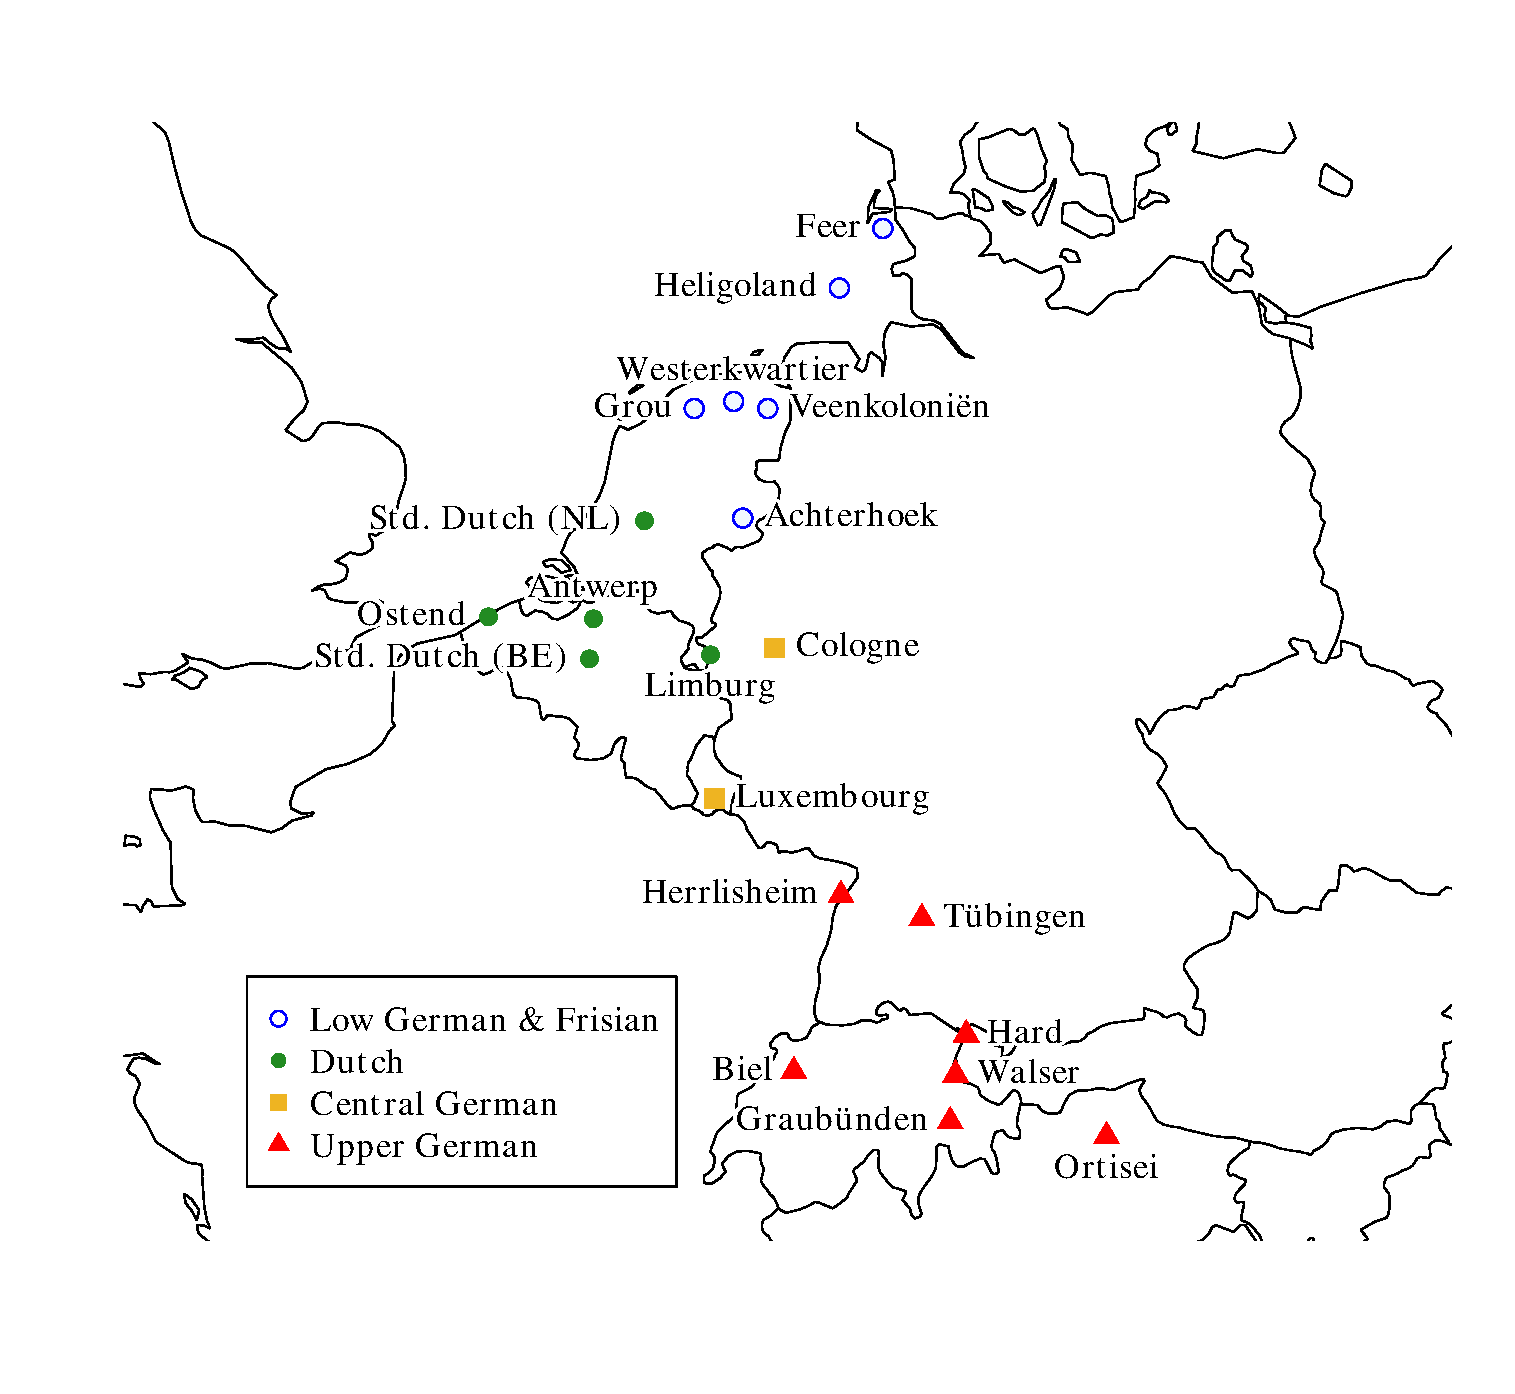
\includegraphics[width=\textwidth]{figures/map.pdf}
\caption
[Locations of the modern continental West Germanic doculects]
{Locations of the modern continental West Germanic doculects we worked with.}
\label{fig:map}
\end{figure}

\begin{figure}[h]
\begin{adjustwidth}{-1cm}{-1cm}
% Importing the dendrograms as PDFs instead of via standalone
% because the latter messes up the placement of the sound corres labels.
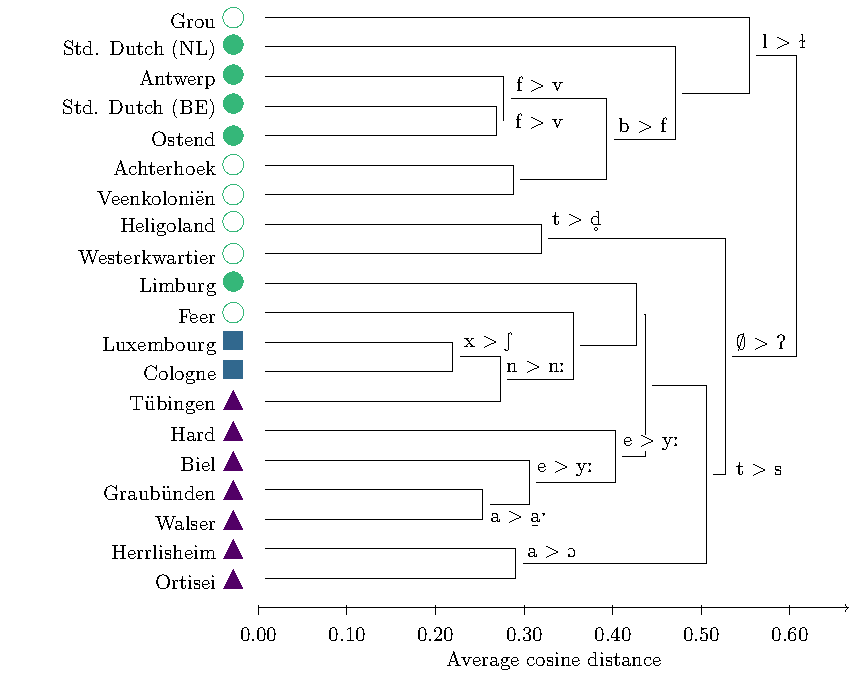
\includegraphics[height=0.45\textheight]{figures/tfidf-nocontext.pdf}\\
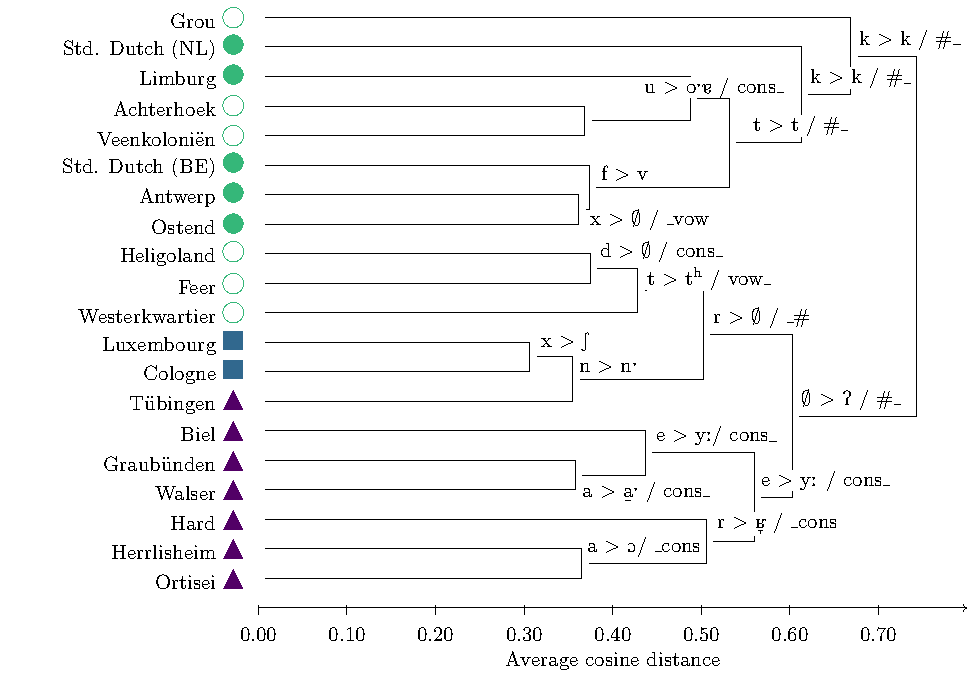
\includegraphics[height=0.45\textheight]{figures/tfidf-context.pdf}
\end{adjustwidth}
\vspace{0.3em}
\begin{center}
{\ingv} Ingv\ae{}onic \hspace{1em}
{\dutch} Dutch \hspace{1em}
{\central} Central German \hspace{1em}
{\upper} Upper German
\end{center}
\caption
[UPGMA with no and with additional context information]
{UPGMA with no (top) and additional (bottom) context information,
as well as the highest-ranking correspondence per non-singleton cluster
(with $\geq$70\% importance).
The sound correspondence rules are explained more thoroughly in the full thesis.
}
\label{fig:tfidf-dendrograms}
\end{figure}

\begin{figure}[h]
\begin{adjustwidth}{-1.5cm}{-1cm}
\centering
\includestandalone[height=0.42\textheight]{figures/bsgc-nocontext}\\
\vspace{1.5em}
\includestandalone[height=0.45\textheight]{figures/bsgc-context}
\end{adjustwidth}

\vspace{0.5em}
\begin{center}
{\ingv} Ingv\ae{}onic \hspace{1em}
{\dutch} Dutch \hspace{1em}
{\central} Central German \hspace{1em}
{\upper} Upper German
\end{center}
\caption
[BSGC with no and with additional context information]
{BSGC with no (top) and additional (bottom) context information,
as well as the highest-ranking correspondence per non-singleton cluster
(with $\geq$70\% importance).
The sound correspondence rules are explained more thoroughly in the full thesis.
}
\label{fig:bsgc-trees}
\end{figure}

\begin{figure}[h]
\begin{adjustwidth}{-2cm}{-2cm}
\centering
\includestandalone[width=0.65\textwidth]{figures/cosine}
\hspace{-7em}
\includestandalone[width=0.65\textwidth]{figures/cosine2}
\end{adjustwidth}
\caption
[Cosine similarities between the doculects (UPGMA-context)]
{
Cosine similarities between the doculects (UPGMA-context).
Lines that are bolder and darker represent greater cosine similarity scores
(i.e. lower cosine distances).
The graphic on the left includes all pairwise similarity scores;
the one on the right only includes the highest 10\% of cosine similarity scores.
}
\label{fig:cosine}
\end{figure}

\bibliographystyle{chicago}
\bibliography{lib}
\end{document}
